\documentclass[10pt]{beamer}\usepackage[]{graphicx}\usepackage[]{color}
%% maxwidth is the original width if it is less than linewidth
%% otherwise use linewidth (to make sure the graphics do not exceed the margin)
\makeatletter
\def\maxwidth{ %
  \ifdim\Gin@nat@width>\linewidth
    \linewidth
  \else
    \Gin@nat@width
  \fi
}
\makeatother

\definecolor{fgcolor}{rgb}{0.345, 0.345, 0.345}
\newcommand{\hlnum}[1]{\textcolor[rgb]{0.686,0.059,0.569}{#1}}%
\newcommand{\hlstr}[1]{\textcolor[rgb]{0.192,0.494,0.8}{#1}}%
\newcommand{\hlcom}[1]{\textcolor[rgb]{0.678,0.584,0.686}{\textit{#1}}}%
\newcommand{\hlopt}[1]{\textcolor[rgb]{0,0,0}{#1}}%
\newcommand{\hlstd}[1]{\textcolor[rgb]{0.345,0.345,0.345}{#1}}%
\newcommand{\hlkwa}[1]{\textcolor[rgb]{0.161,0.373,0.58}{\textbf{#1}}}%
\newcommand{\hlkwb}[1]{\textcolor[rgb]{0.69,0.353,0.396}{#1}}%
\newcommand{\hlkwc}[1]{\textcolor[rgb]{0.333,0.667,0.333}{#1}}%
\newcommand{\hlkwd}[1]{\textcolor[rgb]{0.737,0.353,0.396}{\textbf{#1}}}%
\let\hlipl\hlkwb

\usepackage{framed}
\makeatletter
\newenvironment{kframe}{%
 \def\at@end@of@kframe{}%
 \ifinner\ifhmode%
  \def\at@end@of@kframe{\end{minipage}}%
  \begin{minipage}{\columnwidth}%
 \fi\fi%
 \def\FrameCommand##1{\hskip\@totalleftmargin \hskip-\fboxsep
 \colorbox{shadecolor}{##1}\hskip-\fboxsep
     % There is no \\@totalrightmargin, so:
     \hskip-\linewidth \hskip-\@totalleftmargin \hskip\columnwidth}%
 \MakeFramed {\advance\hsize-\width
   \@totalleftmargin\z@ \linewidth\hsize
   \@setminipage}}%
 {\par\unskip\endMakeFramed%
 \at@end@of@kframe}
\makeatother

\definecolor{shadecolor}{rgb}{.97, .97, .97}
\definecolor{messagecolor}{rgb}{0, 0, 0}
\definecolor{warningcolor}{rgb}{1, 0, 1}
\definecolor{errorcolor}{rgb}{1, 0, 0}
\newenvironment{knitrout}{}{} % an empty environment to be redefined in TeX

\usepackage{alltt}

\usetheme{metropolis}

% Comment out for slides
% \usepackage{pgfpages}
% \pgfpagesuselayout{4 on 1}


\usepackage{booktabs}
\usepackage[scale=2]{ccicons}

\usepackage{pgfplots}
\usepgfplotslibrary{dateplot}

\usepackage{xspace}
\newcommand{\themename}{\textbf{\textsc{metropolis}}\xspace}

\usepackage{color}
\definecolor{LUBlue}{RGB}{0,74,136}
%
\usecolortheme[named=LUBlue]{structure} 
%
%\setbeamercolor*{palette primary}{fg=white, bg=LUBlue}%gray!15!white}
%
%\setbeamercolor{titlelike}{parent=palette primary}
\setbeamercolor{frametitle}{bg=LUBlue}
%\setbeamercolor{frametitle right}{bg=gray!60!white}

\graphicspath{{./figures/}}
\usepackage{booktabs}% http://ctan.org/pkg/booktabs
\usepackage{array}% http://ctan.org/pkg/array
\newcolumntype{M}{>{\centering\arraybackslash}m{\dimexpr.05\linewidth-2\tabcolsep}}

\title{Exploratory Data Analysis}
\subtitle{Part 2: Multivariate graphics + summary statistics}
\date{}
\author{Math 445, Spring 2017}
\titlegraphic{\hfill
\includegraphics[height=1.5cm]{LULogo}}

\usepackage[makeroom]{cancel}
\IfFileExists{upquote.sty}{\usepackage{upquote}}{}
\begin{document}






\maketitle

%\begin{frame}{Overview}
%  \setbeamertemplate{section in toc}[sections numbered]
%  \tableofcontents[hideallsubsections]
%\end{frame}

% ---------------------------------------------------
% ---------------------------------------------------
\section{Plotting multiple variables}

% --------------------------------------------------- Slide --
\begin{frame}[fragile]{Basic bivariate graphics}

\begin{tabular}{ll} \hline
Variable type & Plot suggestions\\\hline
Quantitative vs. quantitative  & Scatterplot\\
    & \\
Quantitative vs. categorical   & Side-by-side boxplots\\
              & Facetted histograms/densities\\
\hline
\end{tabular}

\end{frame}

% --------------------------------------------------- Slide --
\begin{frame}[fragile]{Data: 2012 Olympic Athletes}

\begin{knitrout}\scriptsize
\definecolor{shadecolor}{rgb}{0.969, 0.969, 0.969}\color{fgcolor}\begin{kframe}
\begin{alltt}
\hlstd{oly12} \hlkwb{<-} \hlkwd{read.table}\hlstd{(}\hlstr{"https://raw.githubusercontent.com/math445-LU/2016/master/data/oly12.csv"}\hlstd{,}
    \hlkwc{sep} \hlstd{=} \hlstr{","}\hlstd{,} \hlkwc{header} \hlstd{=} \hlnum{TRUE}\hlstd{)}
\hlstd{oly12}\hlopt{$}\hlstd{Sport} \hlkwb{<-} \hlkwd{abbreviate}\hlstd{(oly12}\hlopt{$}\hlstd{Sport,} \hlnum{12}\hlstd{)}
\hlkwd{str}\hlstd{(oly12)}
\end{alltt}
\end{kframe}
\end{knitrout}


\begin{knitrout}\scriptsize
\definecolor{shadecolor}{rgb}{0.969, 0.969, 0.969}\color{fgcolor}\begin{kframe}
\begin{verbatim}
## 'data.frame':	10384 obs. of  14 variables:
##  $ Name   : Factor w/ 10366 levels "Aaron Brown",..: 5353 121 4117 16 6033 5686 6061 6765 2738 3854 ...
##  $ Country: Factor w/ 205 levels "Afghanistan",..: 144 195 68 125 154 68 8 125 94 3 ...
##  $ Age    : int  23 33 30 24 26 27 30 23 27 19 ...
##  $ Height : num  1.7 1.93 1.87 NA 1.78 1.82 1.82 1.87 1.9 1.7 ...
##  $ Weight : int  60 125 76 NA 85 80 73 75 80 NA ...
##  $ Sex    : Factor w/ 2 levels "F","M": 2 2 2 2 1 2 1 2 2 2 ...
##  $ DOB    : Date, format: "1989-02-06" NA ...
##  $ PlaceOB: Factor w/ 4108 levels "","Aachen (GER)",..: 2486 3302 398 48 3436 1 1 1 1172 2266 ...
##  $ Gold   : int  0 0 0 0 0 0 0 0 0 0 ...
##  $ Silver : int  0 0 0 0 0 0 0 0 0 0 ...
##  $ Bronze : int  0 0 0 0 0 0 0 0 0 0 ...
##  $ Total  : int  0 0 0 0 0 0 0 0 0 0 ...
##  $ Sport  : chr  "Judo" "Athletics" "Athletics" "Boxing" ...
##  $ Event  : Factor w/ 763 levels "Group All-Around",..: 350 405 251 443 699 406 726 403 248 491 ...
\end{verbatim}
\end{kframe}
\end{knitrout}

\end{frame}


% --------------------------------------------------- Slide --
\begin{frame}[fragile]{Scatterplots}
\begin{knitrout}\small
\definecolor{shadecolor}{rgb}{0.969, 0.969, 0.969}\color{fgcolor}\begin{kframe}
\begin{alltt}
\hlkwd{ggplot}\hlstd{(}\hlkwc{data} \hlstd{= oly12,} \hlkwc{mapping} \hlstd{=} \hlkwd{aes}\hlstd{(}\hlkwc{x} \hlstd{= Height,} \hlkwc{y} \hlstd{= Weight))} \hlopt{+}
 \hlkwd{geom_point}\hlstd{()}
\end{alltt}
\end{kframe}
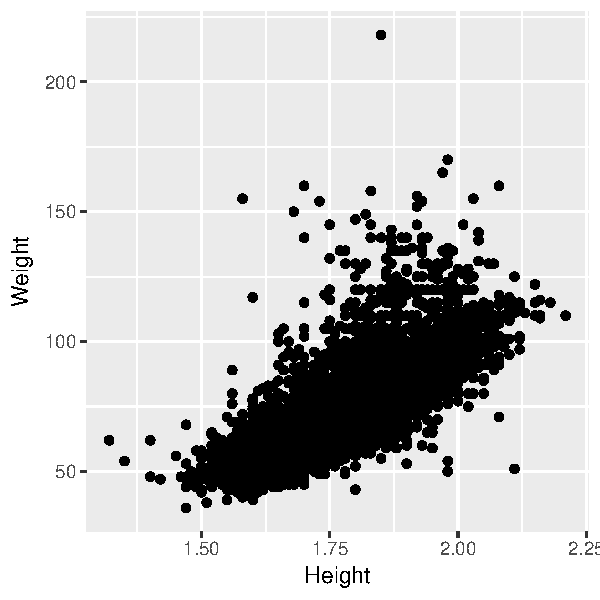
\includegraphics[width=2.5in,height=2.5in]{figure/unnamed-chunk-5-1} 

\end{knitrout}
\end{frame}

% --------------------------------------------------- Slide --
\begin{frame}[fragile]{Scatterplots + Alpha Blending}
\begin{knitrout}\small
\definecolor{shadecolor}{rgb}{0.969, 0.969, 0.969}\color{fgcolor}\begin{kframe}
\begin{alltt}
\hlkwd{ggplot}\hlstd{(}\hlkwc{data} \hlstd{= oly12,} \hlkwc{mapping} \hlstd{=} \hlkwd{aes}\hlstd{(}\hlkwc{x} \hlstd{= Height,} \hlkwc{y} \hlstd{= Weight))} \hlopt{+}
 \hlkwd{geom_point}\hlstd{(}\hlkwc{alpha} \hlstd{=} \hlnum{0.3}\hlstd{)}
\end{alltt}
\end{kframe}
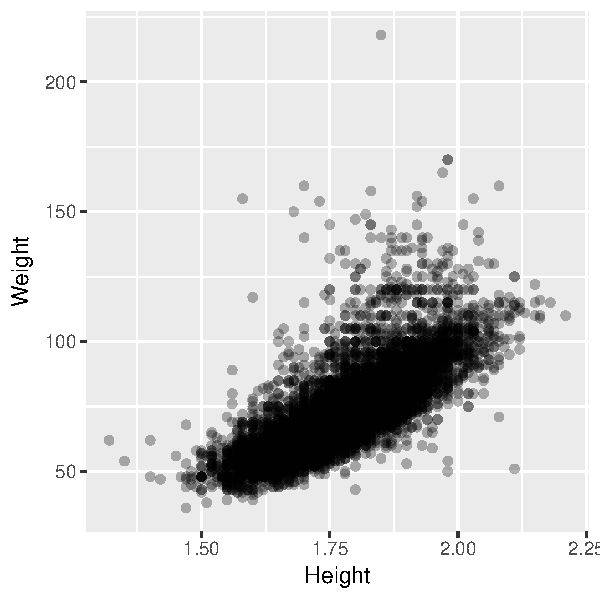
\includegraphics[width=2.5in,height=2.5in]{figure/unnamed-chunk-6-1} 

\end{knitrout}
\end{frame}

% --------------------------------------------------- Slide --
\begin{frame}[fragile]{Scatterplots + Smoother}
\begin{knitrout}\small
\definecolor{shadecolor}{rgb}{0.969, 0.969, 0.969}\color{fgcolor}\begin{kframe}
\begin{alltt}
\hlkwd{ggplot}\hlstd{(}\hlkwc{data} \hlstd{= oly12,} \hlkwc{mapping} \hlstd{=} \hlkwd{aes}\hlstd{(}\hlkwc{x} \hlstd{= Height,} \hlkwc{y} \hlstd{= Weight))} \hlopt{+}
 \hlkwd{geom_point}\hlstd{(}\hlkwc{alpha} \hlstd{=} \hlnum{0.3}\hlstd{)} \hlopt{+}
 \hlkwd{geom_smooth}\hlstd{()}
\end{alltt}
\end{kframe}
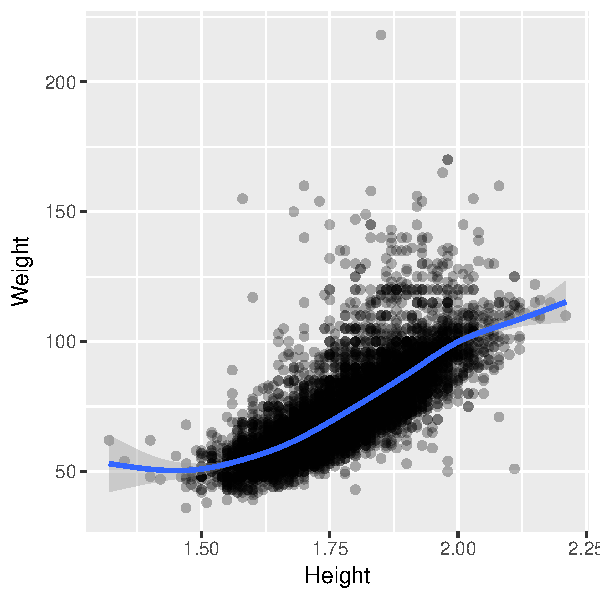
\includegraphics[width=2.5in,height=2.5in]{figure/unnamed-chunk-7-1} 

\end{knitrout}
\end{frame}

% --------------------------------------------------- Slide --
\begin{frame}[fragile]{Scatterplots with extra variables}

\begin{knitrout}\footnotesize
\definecolor{shadecolor}{rgb}{0.969, 0.969, 0.969}\color{fgcolor}\begin{kframe}
\begin{alltt}
\hlkwd{library}\hlstd{(viridis)}
\hlkwd{ggplot}\hlstd{(}\hlkwc{data} \hlstd{= oly12,} \hlkwc{mapping} \hlstd{=} \hlkwd{aes}\hlstd{(}\hlkwc{x} \hlstd{= Height,} \hlkwc{y} \hlstd{= Weight,} \hlkwc{color} \hlstd{= Sex))} \hlopt{+}
  \hlkwd{geom_point}\hlstd{(}\hlkwc{alpha} \hlstd{=} \hlnum{0.3}\hlstd{)} \hlopt{+}
  \hlkwd{scale_color_viridis}\hlstd{(}\hlkwc{discrete} \hlstd{=} \hlnum{TRUE}\hlstd{)}
\end{alltt}
\end{kframe}
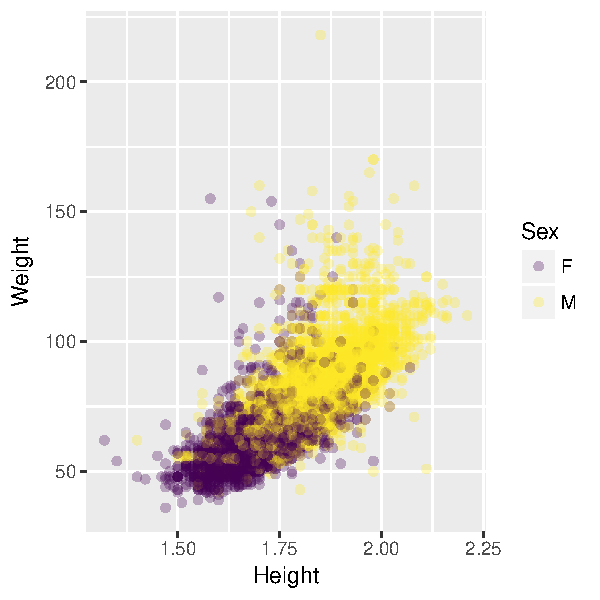
\includegraphics[width=2.75in,height=2.5in]{figure/unnamed-chunk-8-1} 

\end{knitrout}

\end{frame}


% --------------------------------------------------- Slide --
\begin{frame}[fragile]{Side-by-side boxplots}


\begin{knitrout}\scriptsize
\definecolor{shadecolor}{rgb}{0.969, 0.969, 0.969}\color{fgcolor}\begin{kframe}
\begin{alltt}
\hlkwd{ggplot}\hlstd{(}\hlkwc{data} \hlstd{= oly12,} \hlkwc{mapping} \hlstd{=} \hlkwd{aes}\hlstd{(}\hlkwc{x} \hlstd{= Sport,} \hlkwc{y} \hlstd{= Age))} \hlopt{+}
  \hlkwd{geom_boxplot}\hlstd{()} \hlopt{+}
  \hlkwd{coord_flip}\hlstd{()}
\end{alltt}
\end{kframe}
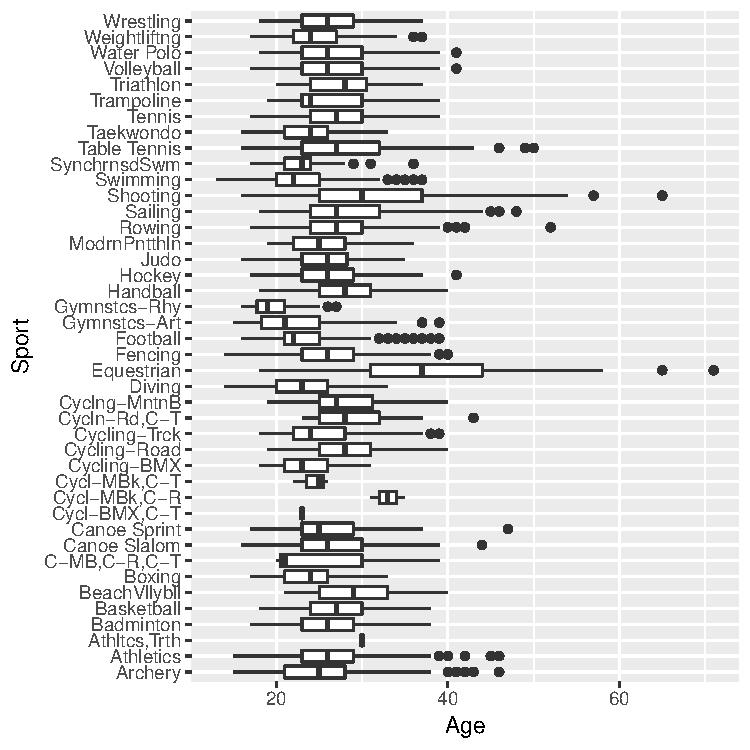
\includegraphics[width=2.5in,height=2.5in]{figure/unnamed-chunk-9-1} 

\end{knitrout}

\end{frame}

% --------------------------------------------------- Slide --
\begin{frame}[fragile]{Side-by-side boxplots}

\begin{knitrout}\scriptsize
\definecolor{shadecolor}{rgb}{0.969, 0.969, 0.969}\color{fgcolor}\begin{kframe}
\begin{alltt}
\hlkwd{ggplot}\hlstd{(}\hlkwc{data} \hlstd{= oly12,} \hlkwc{mapping} \hlstd{=} \hlkwd{aes}\hlstd{(}\hlkwc{x} \hlstd{=} \hlkwd{reorder}\hlstd{(Sport, Age, median),} \hlkwc{y} \hlstd{= Age))} \hlopt{+}
  \hlkwd{geom_boxplot}\hlstd{()} \hlopt{+}
  \hlkwd{coord_flip}\hlstd{()} \hlopt{+}
  \hlkwd{labs}\hlstd{(}\hlkwc{x} \hlstd{=} \hlstr{"Sport"}\hlstd{)}
\end{alltt}
\end{kframe}
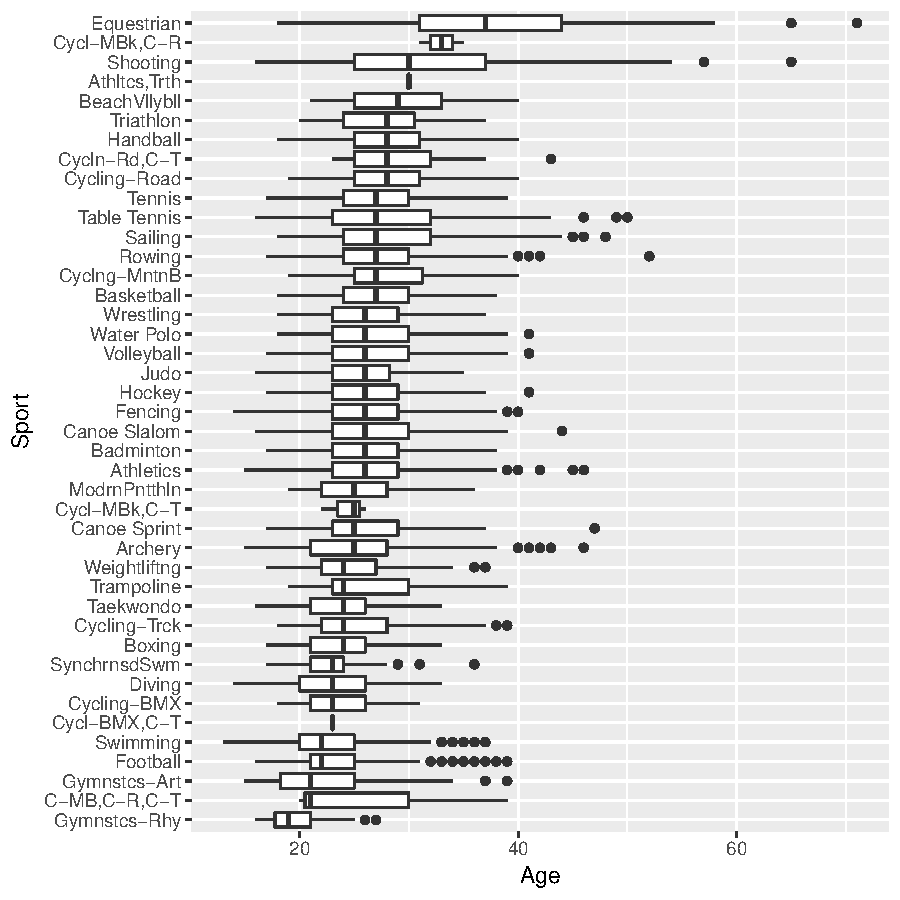
\includegraphics[width=2.75in,height=2.75in]{figure/unnamed-chunk-10-1} 

\end{knitrout}

\end{frame}

% --------------------------------------------------- Slide --
\begin{frame}[fragile]{Facetting}

\begin{knitrout}\scriptsize
\definecolor{shadecolor}{rgb}{0.969, 0.969, 0.969}\color{fgcolor}\begin{kframe}
\begin{alltt}
\hlkwd{ggplot}\hlstd{(}\hlkwc{data} \hlstd{= oly12,} \hlkwc{mapping} \hlstd{=} \hlkwd{aes}\hlstd{(}\hlkwc{x} \hlstd{= Height))} \hlopt{+}
  \hlkwd{geom_histogram}\hlstd{()} \hlopt{+}
  \hlkwd{facet_wrap}\hlstd{(}\hlopt{~} \hlstd{Sport)}
\end{alltt}
\end{kframe}
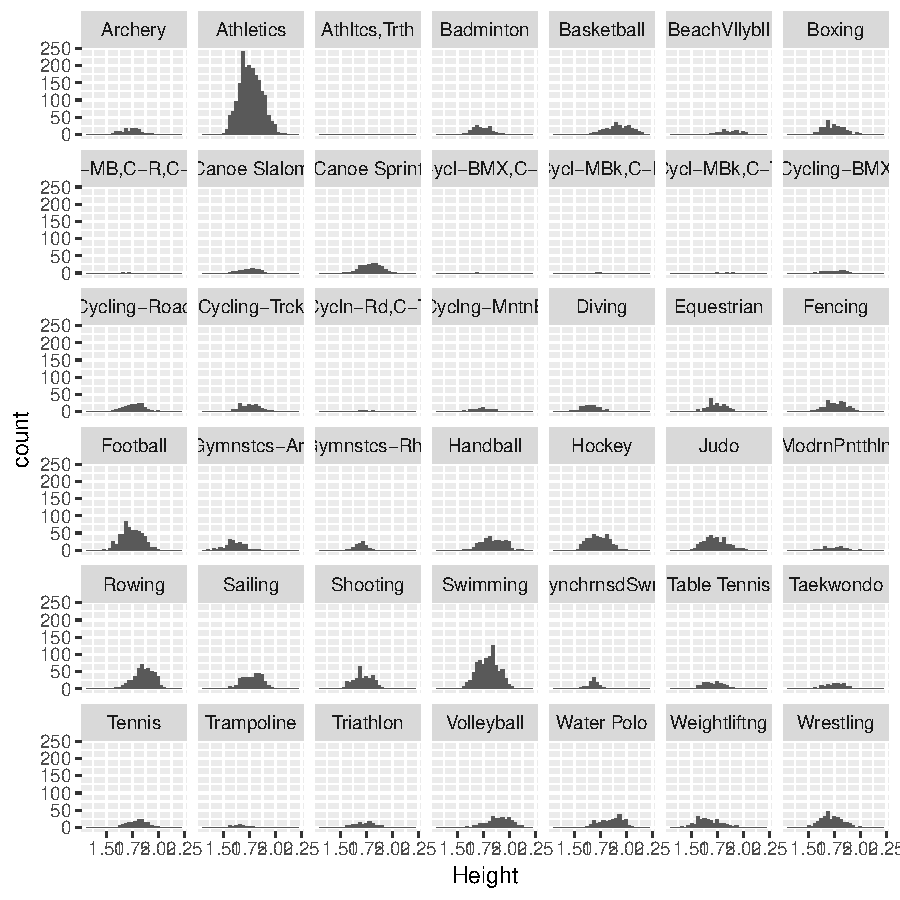
\includegraphics[width=2.75in,height=2.75in]{figure/unnamed-chunk-11-1} 

\end{knitrout}

\end{frame}

% --------------------------------------------------- Slide --
\begin{frame}[fragile]{Facetting}

\begin{knitrout}\scriptsize
\definecolor{shadecolor}{rgb}{0.969, 0.969, 0.969}\color{fgcolor}\begin{kframe}
\begin{alltt}
\hlkwd{ggplot}\hlstd{(}\hlkwc{data} \hlstd{= oly12,} \hlkwc{mapping} \hlstd{=} \hlkwd{aes}\hlstd{(}\hlkwc{x} \hlstd{= Height,} \hlkwc{y} \hlstd{= Weight))} \hlopt{+}
  \hlkwd{geom_point}\hlstd{(}\hlkwc{size} \hlstd{=} \hlnum{1}\hlstd{,} \hlkwc{alpha} \hlstd{=} \hlnum{0.3}\hlstd{)} \hlopt{+}
  \hlkwd{facet_wrap}\hlstd{(}\hlopt{~} \hlstd{Sport)}
\end{alltt}
\end{kframe}
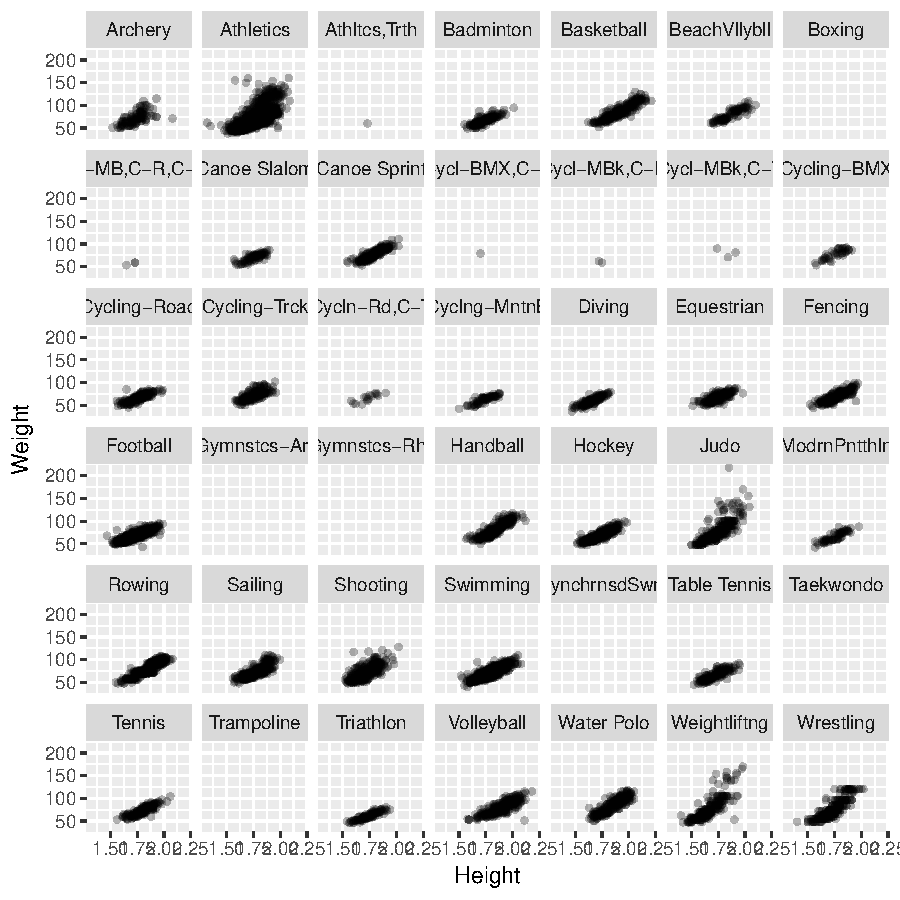
\includegraphics[width=2.75in,height=2.75in]{figure/unnamed-chunk-12-1} 

\end{knitrout}

\end{frame}


% ---------------------------------------------------
% ---------------------------------------------------
\section{Summarizing data numerically}

% --------------------------------------------------- Slide --
\begin{frame}[fragile]{Univariate summaries}

A common way to summarize a variable is to extract the column from the data frame and deal with it separately.

\begin{columns}
\begin{column}{0.3\textwidth}
\begin{knitrout}\scriptsize
\definecolor{shadecolor}{rgb}{0.969, 0.969, 0.969}\color{fgcolor}\begin{kframe}
\begin{alltt}
\hlkwd{mean}\hlstd{(oly12}\hlopt{$}\hlstd{Age)}
\end{alltt}
\begin{verbatim}
## [1] 26.06886
\end{verbatim}
\begin{alltt}
\hlkwd{median}\hlstd{(oly12}\hlopt{$}\hlstd{Age)}
\end{alltt}
\begin{verbatim}
## [1] 25
\end{verbatim}
\begin{alltt}
\hlkwd{sd}\hlstd{(oly12}\hlopt{$}\hlstd{Age)}
\end{alltt}
\begin{verbatim}
## [1] 5.440561
\end{verbatim}
\end{kframe}
\end{knitrout}
\end{column}

\begin{column}{0.5\textwidth}
\begin{knitrout}\scriptsize
\definecolor{shadecolor}{rgb}{0.969, 0.969, 0.969}\color{fgcolor}\begin{kframe}
\begin{alltt}
\hlkwd{var}\hlstd{(oly12}\hlopt{$}\hlstd{Age)}
\end{alltt}
\begin{verbatim}
## [1] 29.59971
\end{verbatim}
\begin{alltt}
\hlkwd{quantile}\hlstd{(oly12}\hlopt{$}\hlstd{Age,} \hlkwc{probs} \hlstd{=} \hlkwd{c}\hlstd{(}\hlnum{0.2}\hlstd{,} \hlnum{0.4}\hlstd{,} \hlnum{0.6}\hlstd{,} \hlnum{0.8}\hlstd{))}
\end{alltt}
\begin{verbatim}
## 20% 40% 60% 80% 
##  22  24  27  30
\end{verbatim}
\end{kframe}
\end{knitrout}
\end{column}
\end{columns}


\end{frame}


% --------------------------------------------------- Slide --
\begin{frame}[fragile]{Summaries by group}

To obtain summaries by group we can use functionality found in the \verb|dplyr| package:

\begin{knitrout}\small
\definecolor{shadecolor}{rgb}{0.969, 0.969, 0.969}\color{fgcolor}\begin{kframe}
\begin{alltt}
\hlcom{# install.packages('dplyr') # uncomment if not installed}
\hlkwd{library}\hlstd{(dplyr)}
\end{alltt}
\end{kframe}
\end{knitrout}

In addition to groupwise processing, \verb|dplyr| provides \alert{chaining syntax}:


\begin{knitrout}\small
\definecolor{shadecolor}{rgb}{0.969, 0.969, 0.969}\color{fgcolor}\begin{kframe}
\begin{alltt}
\hlcom{# Regular (i.e. function application) syntax}
\hlstd{object_name} \hlkwb{<-} \hlkwd{function_name}\hlstd{(}\hlkwc{data} \hlstd{= data_table, arguments)}

\hlcom{# Chaining syntax}
\hlstd{object_name} \hlkwb{<-}
  \hlstd{data_table} \hlopt
  \hlkwd{function_name}\hlstd{(arguments)}
\end{alltt}
\end{kframe}
\end{knitrout}

\end{frame}

% --------------------------------------------------- Slide --
\begin{frame}[fragile]{Summaries by group}

Suppose that we are interested in calculating the average age of 2012 Olympic athletes by sport:

\begin{knitrout}\footnotesize
\definecolor{shadecolor}{rgb}{0.969, 0.969, 0.969}\color{fgcolor}\begin{kframe}
\begin{alltt}
\hlstd{age_sport} \hlkwb{<-}
  \hlstd{oly12} \hlopt
  \hlkwd{group_by}\hlstd{(Sport)} \hlopt
  \hlkwd{summarize}\hlstd{(}\hlkwc{avgAge} \hlstd{=} \hlkwd{mean}\hlstd{(Age))}

\hlkwd{head}\hlstd{(age_sport)}
\end{alltt}
\begin{verbatim}
## # A tibble: 6 × 2
##          Sport   avgAge
##          <chr>    <dbl>
## 1      Archery 26.07438
## 2    Athletics 26.17131
## 3 Athltcs,Trth 30.00000
## 4    Badminton 26.15663
## 5   Basketball 27.17844
## 6 BeachVllybll 29.18280
\end{verbatim}
\end{kframe}
\end{knitrout}

\end{frame}

% --------------------------------------------------- Slide --
\begin{frame}[fragile]{Summaries by group}

We can also quickly obtain the medal count by country:

\begin{knitrout}\footnotesize
\definecolor{shadecolor}{rgb}{0.969, 0.969, 0.969}\color{fgcolor}\begin{kframe}
\begin{alltt}
\hlstd{medal_count} \hlkwb{<-}
  \hlstd{oly12} \hlopt
  \hlkwd{group_by}\hlstd{(Country)} \hlopt
  \hlkwd{summarize}\hlstd{(}\hlkwc{Gold} \hlstd{=} \hlkwd{sum}\hlstd{(Gold),} \hlkwc{Silver} \hlstd{=} \hlkwd{sum}\hlstd{(Silver),} \hlkwc{Bronze} \hlstd{=} \hlkwd{sum}\hlstd{(Bronze))} \hlopt
  \hlkwd{arrange}\hlstd{(}\hlkwd{desc}\hlstd{(Gold),} \hlkwd{desc}\hlstd{(Silver),} \hlkwd{desc}\hlstd{(Bronze))}

\hlkwd{head}\hlstd{(medal_count)}
\end{alltt}
\begin{verbatim}
## # A tibble: 6 × 4
##                      Country  Gold Silver Bronze
##                       <fctr> <int>  <int>  <int>
## 1   United States of America    40     19     20
## 2 People's Republic of China    25     15     13
## 3                    Germany    21     11      8
## 4              Great Britain    11     13     20
## 5                     France    11     11     11
## 6          Republic of Korea    10      2     10
\end{verbatim}
\end{kframe}
\end{knitrout}

\end{frame}

% --------------------------------------------------- Slide --
\begin{frame}[fragile]{Subsetting}

What if you only want summaries for one group?

\begin{itemize}
\item Create the summaries for all of the groups and then extract the group of interest
\item Extract data for the group of interest and then create summaries
\end{itemize}

The \verb|filter| command in the \verb|dplyr| package allows you to easily subset a data frame:

\begin{knitrout}\small
\definecolor{shadecolor}{rgb}{0.969, 0.969, 0.969}\color{fgcolor}\begin{kframe}
\begin{alltt}
\hlkwd{filter}\hlstd{(data, criteria)}
\end{alltt}
\end{kframe}
\end{knitrout}

\end{frame}

% --------------------------------------------------- Slide --
\begin{frame}[fragile]{Subsetting}

\begin{knitrout}\small
\definecolor{shadecolor}{rgb}{0.969, 0.969, 0.969}\color{fgcolor}\begin{kframe}
\begin{alltt}
\hlstd{oly12} \hlopt
  \hlkwd{filter}\hlstd{(Country} \hlopt{==} \hlstr{"United States of America"}\hlstd{)} \hlopt
  \hlkwd{group_by}\hlstd{(Sex)} \hlopt
  \hlkwd{summarize}\hlstd{(}\hlkwc{avgAge} \hlstd{=} \hlkwd{mean}\hlstd{(Age))}
\end{alltt}
\begin{verbatim}
## # A tibble: 2 × 2
##      Sex   avgAge
##   <fctr>    <dbl>
## 1      F 26.44528
## 2      M 27.73123
\end{verbatim}
\end{kframe}
\end{knitrout}


\end{frame}


% --------------------------------------------------- Slide --
\begin{frame}[fragile]{Subsetting}

\begin{knitrout}\footnotesize
\definecolor{shadecolor}{rgb}{0.969, 0.969, 0.969}\color{fgcolor}\begin{kframe}
\begin{alltt}
\hlstd{oly12} \hlopt
  \hlkwd{filter}\hlstd{(Gold} \hlopt{>} \hlnum{0} \hlopt{|} \hlstd{Silver} \hlopt{>} \hlnum{0} \hlopt{|} \hlstd{Bronze} \hlopt{>} \hlnum{0}\hlstd{)} \hlopt
  \hlkwd{ggplot}\hlstd{(}\hlkwc{mapping} \hlstd{=} \hlkwd{aes}\hlstd{(}\hlkwc{x} \hlstd{= Age,} \hlkwc{group} \hlstd{= Sex,} \hlkwc{fill} \hlstd{= Sex))} \hlopt{+}
  \hlkwd{geom_density}\hlstd{(}\hlkwc{alpha} \hlstd{=} \hlnum{0.5}\hlstd{)}
\end{alltt}
\end{kframe}
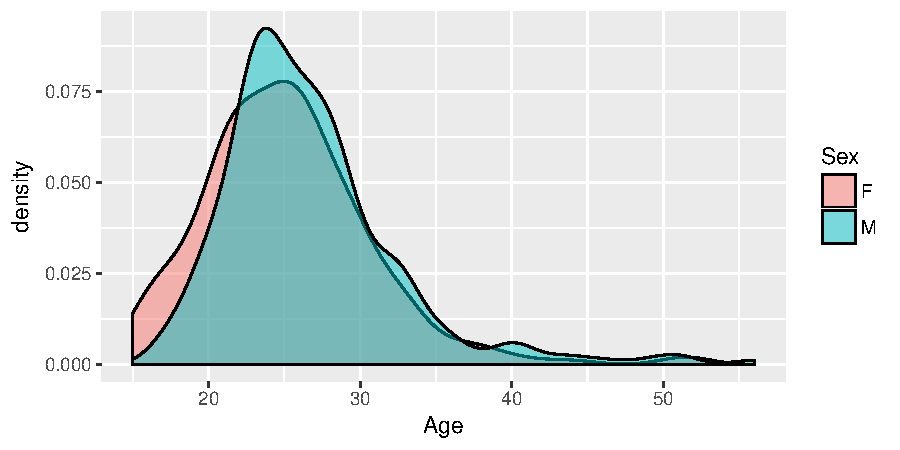
\includegraphics[width=3in,height=2in]{figure/unnamed-chunk-21-1} 

\end{knitrout}

\end{frame}



\end{document}
